% https://es.overleaf.com/latex/templates/project-report/jpzczmpsdzwm

%%% Preamble
\documentclass[paper=leter, fontsize=11pt]{scrartcl}
\usepackage[utf8]{inputenc}
\usepackage[spanish,mexico]{babel}
\usepackage[T1]{fontenc}    % use 8-bit T1 fonts
\usepackage{lmodern}
\usepackage{hyperref}       % hyperlinks
\usepackage{lipsum}
\usepackage[square,numbers]{natbib}

\usepackage[protrusion=true,expansion=true]{microtype}	
\usepackage{amsmath,amsfonts,amsthm} % Math packages
\usepackage[pdftex]{graphicx}
\usepackage{url}
 
\usepackage{booktabs}
\usepackage[table,xcdraw]{xcolor}

\usepackage{tikz}
\usetikzlibrary{positioning,matrix, arrows.meta}

\usepackage{caption} 
\usepackage{subcaption}

\usepackage{listings}
\lstdefinestyle{mystyle}{
    basicstyle=\ttfamily\footnotesize,
    breakatwhitespace=false,         
    breaklines=true,                 
    captionpos=b,                    
    keepspaces=true,                 
    numbers=left,                    
    numbersep=5pt,                  
    showspaces=false,                
    showstringspaces=false,
    showtabs=false,                  
    tabsize=4
}

\lstset{style=mystyle}
\renewcommand{\lstlistingname}{Código}

\graphicspath{ {imgs/} }

\selectlanguage{spanish}
\usepackage[spanish,onelanguage,ruled]{algorithm2e}


%%% Custom sectioning
\usepackage{sectsty}
\allsectionsfont{\centering \normalfont\scshape}


%%% Custom headers/footers (fancyhdr package)
\usepackage{fancyhdr}
\pagestyle{fancyplain}
\fancyhead{}											% No page header
\fancyfoot[L]{}											% Empty 
\fancyfoot[C]{}											% Empty
\fancyfoot[R]{\thepage}									% Pagenumbering
\renewcommand{\headrulewidth}{0pt}			% Remove header underlines
\renewcommand{\footrulewidth}{0pt}				% Remove footer underlines
\setlength{\headheight}{13.6pt}


%%% Equation and float numbering
\numberwithin{equation}{section}		% Equationnumbering: section.eq#
\numberwithin{figure}{section}			% Figurenumbering: section.fig#
\numberwithin{table}{section}				% Tablenumbering: section.tab#


%%% Maketitle metadata
\newcommand{\horrule}[1]{\rule{\linewidth}{#1}} 	% Horizontal rule

%%% https://tex.stackexchange.com/a/118217
\usepackage{mathtools}
\DeclarePairedDelimiter\ceil{\lceil}{\rceil}
\DeclarePairedDelimiter\floor{\lfloor}{\rfloor}

\usepackage{amsmath}

\usepackage{tikz}

\title{
		%\vspace{-1in} 	
		\usefont{OT1}{bch}{b}{n}
		\normalfont \normalsize \textsc{Posgrado de Ingeniería de Sistemas} \\ [25pt]
		\horrule{0.5pt} \\[0.4cm]
		\huge Conceptos básicos de probabilidad \\
		\horrule{2pt} \\[0.5cm]
}
\author{
		\normalfont 								\normalsize
        Alberto Benavides\\[-3pt]		\normalsize
        \today
}
\date{}


%%% Begin document
\begin{document}
\maketitle

\section{Sobre los datos}

En este reporte se estudia la estadística descriptiva básica de los datos de cantidad de derechohabientes en las instituciones de salud de México durante 2015. Los datos fueron obtenidos del INEGI \cite{datos}. Un ejemplo de estos datos se muestra en el cuadro \ref{ejemplo}.

\begin{table}[]
    \resizebox{\textwidth}{!}{%
        \begin{tabular}{@{}lrrrrrr@{}}
        \toprule
        \multicolumn{1}{c}{\textbf{Lugar}} & \multicolumn{1}{c}{\textbf{IMSS}} & \multicolumn{1}{c}{\textbf{ISSSTE}} & \multicolumn{1}{c}{\textbf{PEMEX}} & \multicolumn{1}{c}{\textbf{S. P.}} & \multicolumn{1}{c}{\textbf{Privada}} & \multicolumn{1}{c}{\textbf{Otras}} \\ \midrule
        Michoacán de Ocampo & 954244 & 265494 & 13068 & 2154013 & 52033 & 26847 \\
        Nuevo León & 2973597 & 197764 & 21941 & 905381 & 424545 & 137741 \\
        Durango & 620648 & 182302 & 9135 & 672183 & 21418 & 9999 \\ \bottomrule
        \end{tabular}%
    }
    \caption{Ejemplo de datos obtenidos del INEGI que contienen la cantidad de derechohabientes por institución de salud en México durante 2015.}
    \label{ejemplo}
\end{table}

Para el análisis de estos datos, se ha elegido el uso del programa R versión 4.0.2 \cite{r} que se ejecuta en un entorno de Jupyter \cite{jupyter} que se encuentra disponible en \url{https://tinyurl.com/y52zhl5c}.

Los datos obtenidos de la página del INEGI están en formato \texttt{XLSX}, los cuales se editaron con Microsoft Excel \cite{excel} para obtener sólo las instituciones y los estados donde se presentan. Los estados son todos los de la república mexicana, mientras que las instituciones son el IMMS, el ISSSTE, las afiliadas a PEMEX, el Seguro Popular y sus derivados actuales y, por último, las instituciones privadas.

\section{Representación gráfica}

Una manera visualmente directa de conocer los datos consiste en crear un diagrama de cajas y bigotes. Estos diagramas resumen la información al graficar el mínimo, máximo, media, primer cuartil y tercer cuartil de los datos. En la imagen \ref{inst} (p. \pageref{inst}) puede verse este diagrama de la derechohabiencia por institución en México. Cuando las cajas están muy cercanas entre sí, suele convenir hacer un diagrama de cajas y bigotes en escala logarítmica, como se muestra en la imagen \ref{inst_log} (p. \pageref{inst_log}). A partir de estos diagramas se puede ver que el IMSSS y el seguro popular son las instituciones con más afiliados. Cabe mencionar que es posible que los afiliados de una institución también lo sean de otras.

\begin{figure}
    \centering
    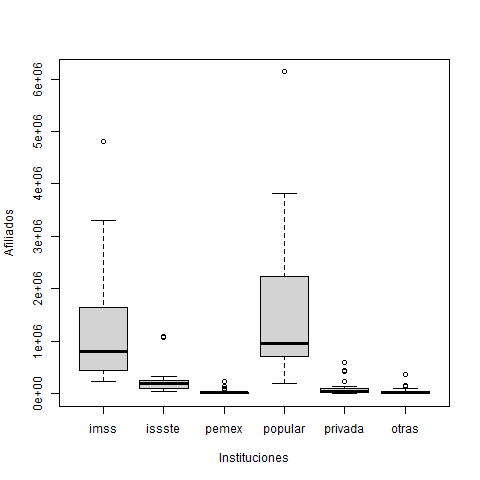
\includegraphics[width=0.8\textwidth]{inst.png}
    \caption{Diagramas de cajas y bigotes de la cantidad de derechohabientes por institución de salud en México durante 2015.}
    \label{inst}
\end{figure}

\begin{figure}
    \centering
    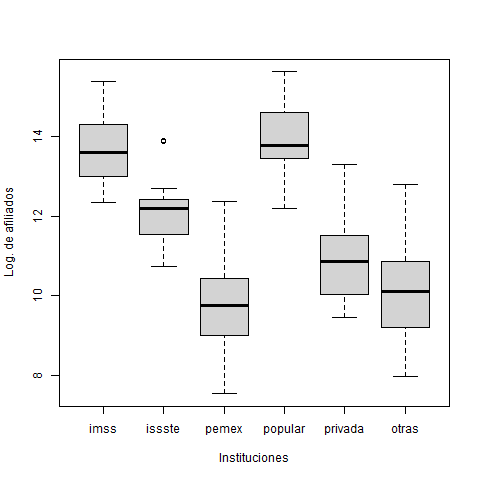
\includegraphics[width=0.8\textwidth]{inst_log.png}
    \caption{Diagramas de cajas y bigotes del logaritmo de la cantidad de derechohabientes por institución de salud en México durante 2015.}
    \label{inst_log}
\end{figure}

Finalmente, también puede obtenerse el diagrama de cajas y bigotes por estado. Éstos se presentan en la figura \ref{estados} (p. \pageref{estados}). En ésta se puede constatar que entre la Ciudad de México y el estado de México existe una gran cantidad de afiliados.

\begin{figure}
    \centering
    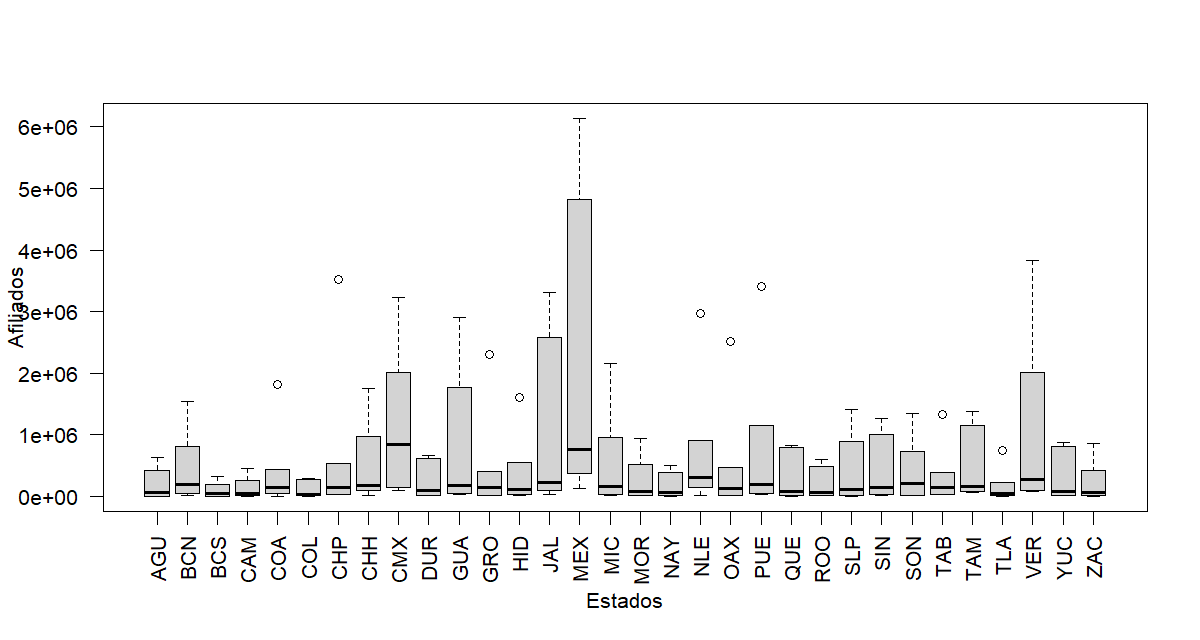
\includegraphics[width=1\textwidth]{estados.png}
    \caption{Diagramas de cajas y bigotes de la cantidad de derechohabientes por estado de México durante 2015. Los nombres de los estados aparecen abreviados conforme al código ISO 3166-2:MX \cite{iso}.} 
    \label{estados}
\end{figure}

\bibliographystyle{plainnat}
\bibliography{Biblio}

\end{document}